% Options for packages loaded elsewhere
\PassOptionsToPackage{unicode}{hyperref}
\PassOptionsToPackage{hyphens}{url}
%
\documentclass[
]{article}
\usepackage{lmodern}
\usepackage{amssymb,amsmath}
\usepackage{ifxetex,ifluatex}
\ifnum 0\ifxetex 1\fi\ifluatex 1\fi=0 % if pdftex
  \usepackage[T1]{fontenc}
  \usepackage[utf8]{inputenc}
  \usepackage{textcomp} % provide euro and other symbols
\else % if luatex or xetex
  \usepackage{unicode-math}
  \defaultfontfeatures{Scale=MatchLowercase}
  \defaultfontfeatures[\rmfamily]{Ligatures=TeX,Scale=1}
\fi
% Use upquote if available, for straight quotes in verbatim environments
\IfFileExists{upquote.sty}{\usepackage{upquote}}{}
\IfFileExists{microtype.sty}{% use microtype if available
  \usepackage[]{microtype}
  \UseMicrotypeSet[protrusion]{basicmath} % disable protrusion for tt fonts
}{}
\makeatletter
\@ifundefined{KOMAClassName}{% if non-KOMA class
  \IfFileExists{parskip.sty}{%
    \usepackage{parskip}
  }{% else
    \setlength{\parindent}{0pt}
    \setlength{\parskip}{6pt plus 2pt minus 1pt}}
}{% if KOMA class
  \KOMAoptions{parskip=half}}
\makeatother
\usepackage{xcolor}
\IfFileExists{xurl.sty}{\usepackage{xurl}}{} % add URL line breaks if available
\IfFileExists{bookmark.sty}{\usepackage{bookmark}}{\usepackage{hyperref}}
\hypersetup{
  pdftitle={Selecting and ranking interesting pairs of cyclic temporal granularities},
  hidelinks,
  pdfcreator={LaTeX via pandoc}}
\urlstyle{same} % disable monospaced font for URLs
\usepackage[margin=1in]{geometry}
\usepackage{longtable,booktabs}
% Correct order of tables after \paragraph or \subparagraph
\usepackage{etoolbox}
\makeatletter
\patchcmd\longtable{\par}{\if@noskipsec\mbox{}\fi\par}{}{}
\makeatother
% Allow footnotes in longtable head/foot
\IfFileExists{footnotehyper.sty}{\usepackage{footnotehyper}}{\usepackage{footnote}}
\makesavenoteenv{longtable}
\usepackage{graphicx,grffile}
\makeatletter
\def\maxwidth{\ifdim\Gin@nat@width>\linewidth\linewidth\else\Gin@nat@width\fi}
\def\maxheight{\ifdim\Gin@nat@height>\textheight\textheight\else\Gin@nat@height\fi}
\makeatother
% Scale images if necessary, so that they will not overflow the page
% margins by default, and it is still possible to overwrite the defaults
% using explicit options in \includegraphics[width, height, ...]{}
\setkeys{Gin}{width=\maxwidth,height=\maxheight,keepaspectratio}
% Set default figure placement to htbp
\makeatletter
\def\fps@figure{htbp}
\makeatother
\setlength{\emergencystretch}{3em} % prevent overfull lines
\providecommand{\tightlist}{%
  \setlength{\itemsep}{0pt}\setlength{\parskip}{0pt}}
\setcounter{secnumdepth}{5}
\usepackage{booktabs}
\usepackage{longtable}
\usepackage{array}
\usepackage{multirow}
\usepackage{wrapfig}
\usepackage{float}
\usepackage{colortbl}
\usepackage{pdflscape}
\usepackage{tabu}
\usepackage{threeparttable}
\usepackage{threeparttablex}
\usepackage[normalem]{ulem}
\usepackage{makecell}

\title{Selecting and ranking interesting pairs of cyclic temporal granularities}
\author{}
\date{\vspace{-2.5em}}

\begin{document}
\maketitle

{
\setcounter{tocdepth}{2}
\tableofcontents
}
\hypertarget{introduction}{%
\section{Introduction}\label{introduction}}

Exploratory data analysis, as coined by John W. Tukey (Tukey 1965) involves many iterations of finding structures and patterns that allows the data to be informative. With temporal data available at finer scales, exploring periodicity and their relationships can become overwhelming with so many possible cyclic temporal granularities (Gupta et al. 2020) to explore.

\begin{figure}

{\centering 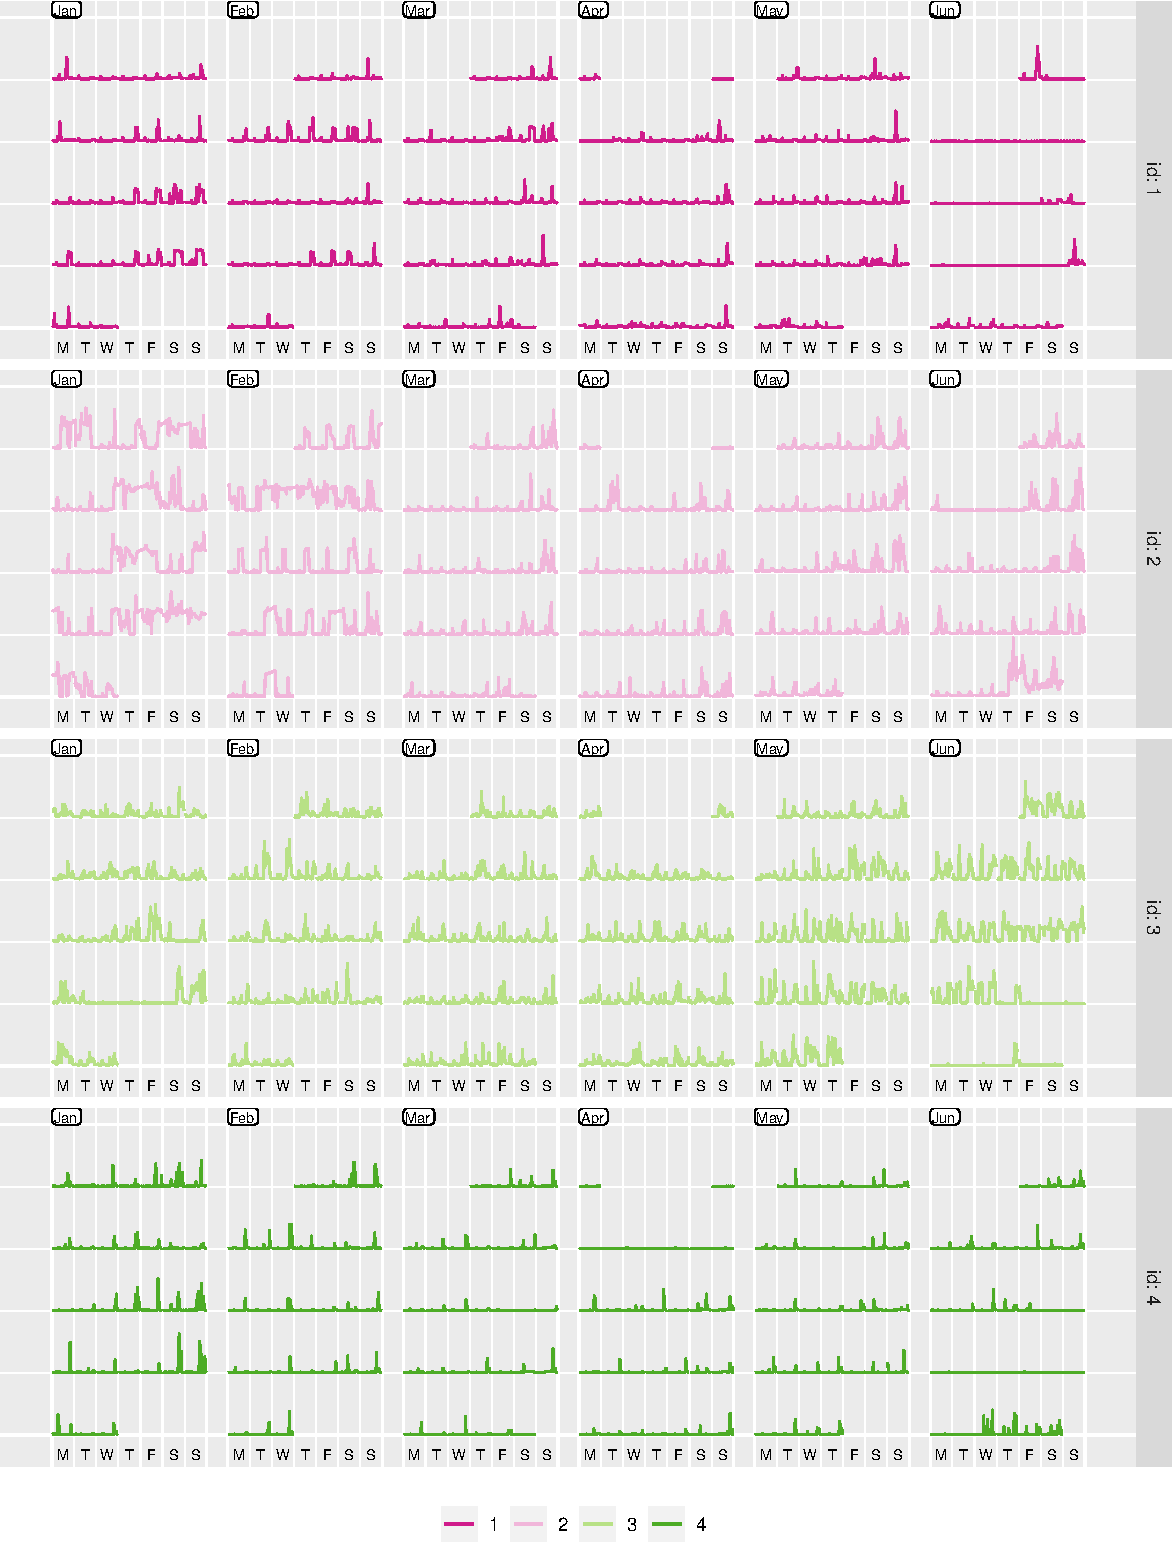
\includegraphics[width=\textwidth]{figure/calendar-elec-1} 

}

\caption{Calendar display.}\label{fig:calendar-elec}
\end{figure}

\noindent Take the example of the calendar display of electricity smart meter data (\ref{fig:calendar-elec}) used in Wang, Cook, and Hyndman (2020) for four households in Melbourne, Australia. The authors show how hour-of-the-day interact with weekday and weekends and then move on to use calendar display to show daily schedules. The calendar display has several components in it, which helps us look at energy consumption across hour-of-the-day, day-of-the-week, week-of-the-month, and month-of-the-year at once. Some interaction of these cyclic granularities could also be interpreted from this display. This is a great start to have an overview of the energy consumption. However, if one wants to understand the periodicities in energy behavior and how the periodicities interact in greater details, it is not easy to comprehend the interactions of some periodicities' from this display, due to the combination of linear and cyclic representation of time. For example, this display might not be the best to understand how hour-of-the-day varies and month-of-year varies across week-of-the-month. Further, it is not clear what all interactions of cyclic granularities should be read from this display as there could be many combinations that one can look at. Moreover, calendar effects are not restricted to conventional day-of-week or month-of-year deconstructions (Gupta et al. (2020)) and could include other cyclic granularities like hour-of-week or day-of-fortnight, which could potentially become useful depending on the context.

\begin{figure}

{\centering 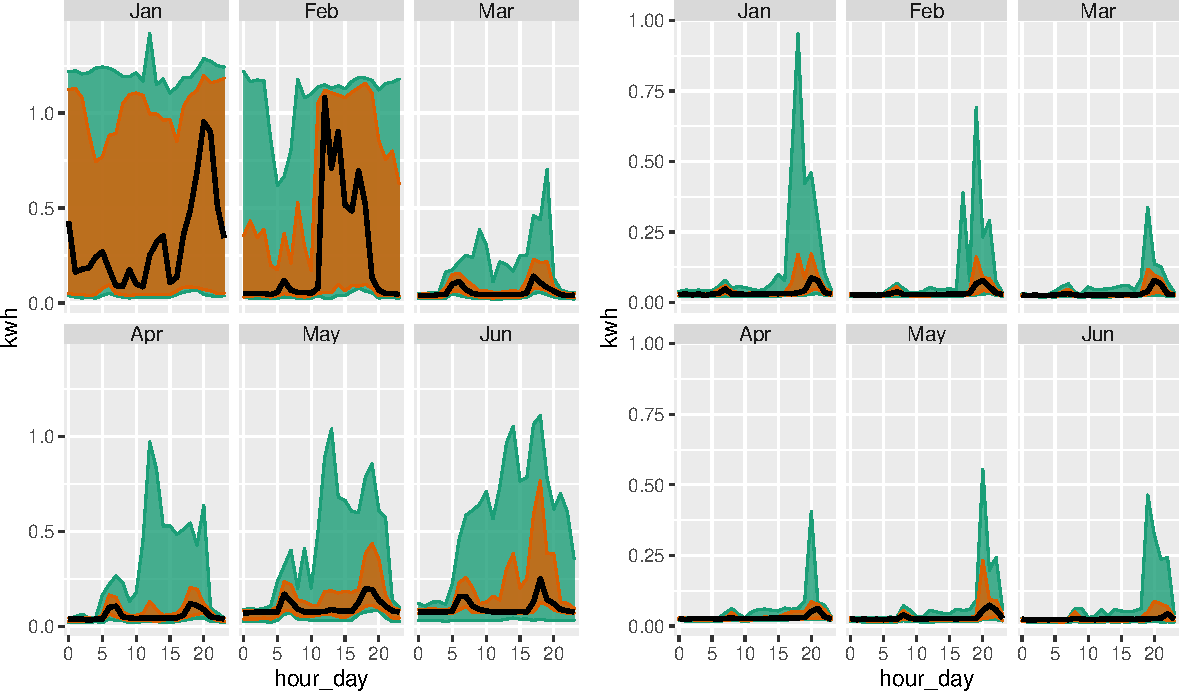
\includegraphics[width=\textwidth]{figure/id2-1} 

}

\caption{something}\label{fig:id2}
\end{figure}

\begin{figure}

{\centering 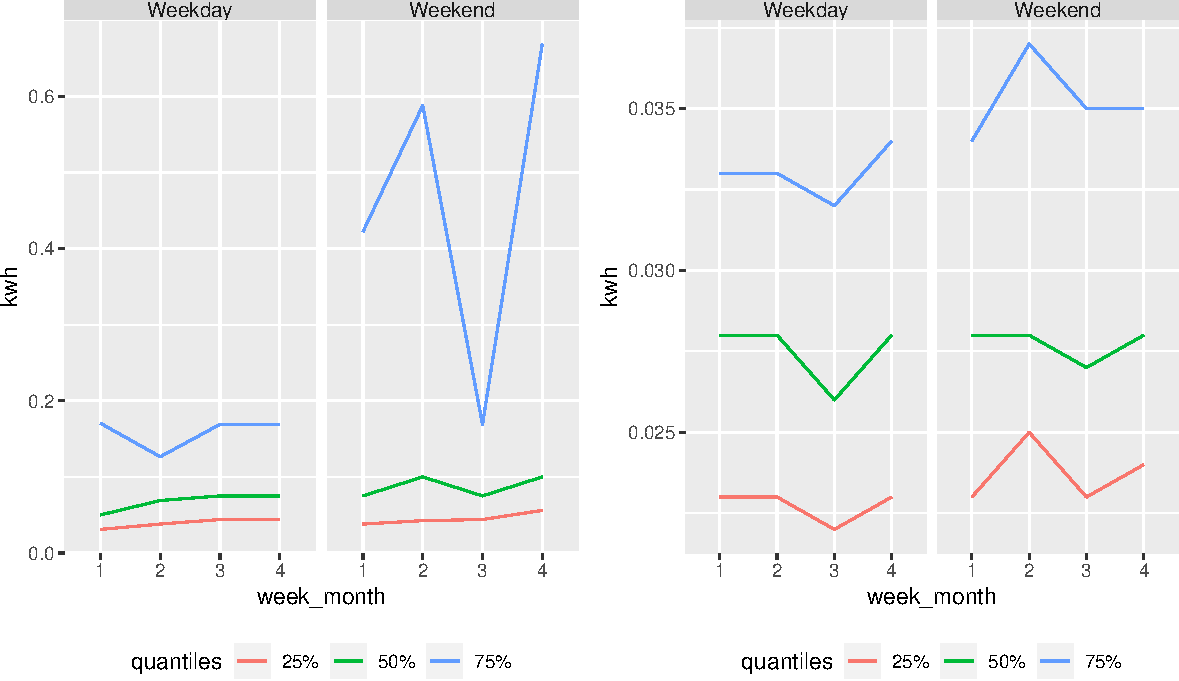
\includegraphics[width=\textwidth]{figure/id4-1} 

}

\caption{something2}\label{fig:id4}
\end{figure}

Moreover, there might be specific interactions that are interesting and others that are not and that too will vary with different households. For example, area distribution quantiles are plotted for household 2 and 4 in Figure \ref{fig:id2}a and b respectively. For the first household, the 75th and 90th percentile for Jan, Feb and July are very close, implying that energy usage for these months are generally on a much higher side due to the usage of air conditioners (in Jan and Feb) and heaters (in July). The energy consumption for household 2 is also higher relative to its own consumption for Jan, Feb and March but the 75th and 90th percentile are apart implying that contrary to the first household, the second household resorts to air conditioners and heaters much less regularly than the first one. Moreover, the 75th percentile distribution is not bimodal across hours of the day for the first household in those months, but the distribution looks similar for all months for the second household. Difference in the energy consumption seem to be varying both across month-of-year (facets) and hour-of-day (x-axis). And thus, both the cyclic granularities would deem important while studying the periodicities in the first household. However, it seems like energy consumption across hours of the day are not that different across different months for the second household. Differences seem to be more prominent across month-of-year (facets) than hour-of-day (x-axis). Again, look at \ref{fig:} c and d, where energy consumption for these two households are plotted against (weekend/weekday, week-of-month). Here, for both households, the pattern of energy consumption vary across different weeks of the month irrespective of the fact it is a weekday or weekend. In that respect, the harmony pair (month-of-year, hour-of-day) seems to be more informative than (weekend/weekday, week-of-month) for the first household. It could be immensely useful to make the transition from all possible ways to only ways that could potentially be informative given a household.

The paper Gupta et al. (2020) describes how we can compute all possible combinations of cyclic time granularities. If we have \(n\) periodic linear granularities in the hierarchy table, then \(n(n-1)/2\) circular or quasi-circular cyclic granularities could be constructed. Let \(N_C\) be the total number of contextual circular, quasi-circular and aperiodic cyclic granularities that can originate from the underlying periodic and aperiodic linear granularities. The mapping of the graphical elements chosen in the paper implies that, for a numeric response variable, the graphics display distributions across combinations of cyclic granularities, one placed at x-axis and the other on the facet. That essentially implies there are \(^{N_C}P_2\) possible pairwise plots exhaustively, where each plot would display a pair of cyclic granularities. This is large and overwhelming for human consumption.

This is similar to Scagnostics (Scatterplot Diagnostics) by Tukey and Tukey (1988), which is used to discern meaningful patterns in large collections of scatterplots. Given a set of \(v\) variables, there are \(v(v-1)/2\) pairs of variables, and thus the same number of possible pairwise scatterplots. Therefore
for even small \(v\), the number of scatterplots can be
large, and scatterplot matrices (SPLOMs) could easily run out of pixels when presenting high-dimensional data. Dang and Wilkinson (2014) and Wilkinson, Anand, and Grossman (2005) provides potential solutions to this, where few characterizations help us to locate anomalies for defining several measures aimed to detect anomalies in density, shape, trend, and
other features in the 2D point scatters.

The paper (Gupta et al. (2020)) narrows down the search from \(^{N_C}P_2\) plots by identifying pairs of granularities that can be meaningfully examined together (a ``harmony''), or when they cannot (a ``clash''). However, even after excluding clashes, the list of harmonies left could be enormous for exhaustive exploration. Hence, there is a need to reduce the search even further by including only those harmonies which are informative enough. Also, ranking the remaining harmony pairs based on how well they capture the variation in the measured variable could be potentially useful.

In this paper, we aim to build a new measure to follow through these two main objectives:

\begin{itemize}
\tightlist
\item
  To choose harmonies for which distributions of categories are significantly different
\item
  To rank the selected harmonies from highest to lowest variation in the distribution of their categories.
\end{itemize}

\hypertarget{median-maximum-pairwise-distances-mmpd}{%
\section{Median Maximum Pairwise Distances (MMPD)}\label{median-maximum-pairwise-distances-mmpd}}

We are interested in assessing structure in probability distributions of the measured variable across bivariate cyclic granularities. We propose a measure called Median Maximum Pairwise Distances (MMPD) to evaluate structure in such a design.

\hypertarget{idea}{%
\subsection{Idea}\label{idea}}

The principle employed for building a new metric is explained through a simple example explained in Figure \ref{fig:null4by2}. Each of these figures have the same panel design with 2 x-axis categories and 4 facet levels. Figure \ref{fig:null4by2}a has all x categories drawn from N(5, 10) distribution for each facet. It is not an interesting display particularly, as distributions do not vary across x-axis or facet categories. Figure \ref{fig:null4by2}b has x categories drawn from the same distribution within a facet and different for different facet categories. Figure \ref{fig:null4by2}b exhibits an exact opposite situation where distribution between the x-axis categories within each facet is different but they are same across facets. Figure \ref{fig:null4by2}d takes a step further by varying the distribution across both facet and x-axis categories. If we are asked to rank the displays in order of importance from minimum to maximum, we might order it as a, b, c and then d.~It might be argued that it is not clear if b should precede or succeed c.~Gestalt theory suggests that when items are placed in close proximity, people assume that they are in the same group because they are close to one another and apart from other groups. Hence, displays that capture more variation within different categories in the same group would be important to bring out different patterns of the data. With this principle, display b could be considered less informative as compared to display c.

With reference to the graphical design in \ref{@Gupta2020-vo}, therefore the idea would be to rate a harmony pair higher if the variation between different levels of the x-axis variable is higher on an average across all levels of the facet variables. Thus the metric could be obtained by computing maximum pairwise distances between distributions of the continuous random variable across x-axis categories for all facets and then taking the median of those maximum pairwise distances across facets. This would help capture the average maximum difference in distribution of the measurement variable explained by the two cyclic granularities together. We call this metric MMPD which stands for Median Maximum Pairwise Distances. In the next section we shall see how we go about computing this measure.

\begin{figure}

{\centering 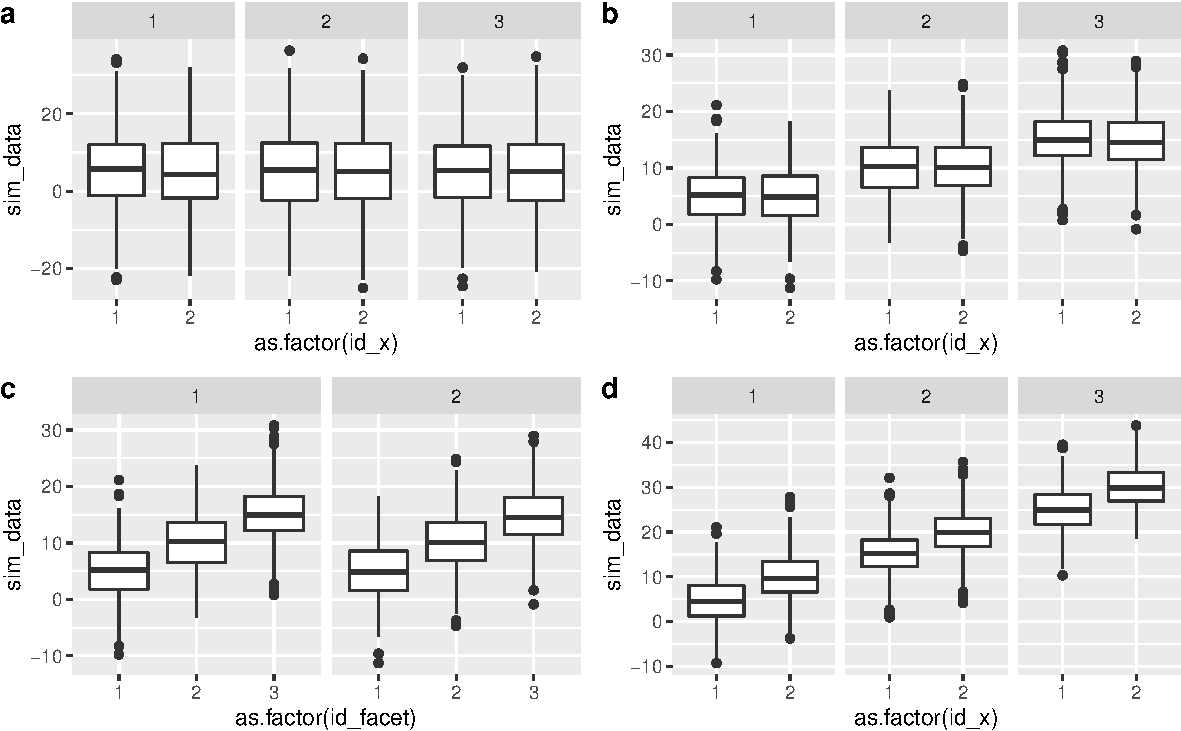
\includegraphics[width=\textwidth]{figure/null4by2-1} 

}

\caption{ A graphical display with two categories mapped to x-axis and 4 categories mapped to facets with the distribution of a continuous random variable plotted on the y-axis. Display a is not interesting as the distribution of the continuous rv does not depend across x-axis or facet categories. Display b and c are more interesting than a since there is a change in distribution either across facets(b) or x-axis(a). Display d is most interesting as distribution of the rv changes across both facet and x-axis variable.}\label{fig:null4by2}
\end{figure}

\hypertarget{computation}{%
\subsection{Computation}\label{computation}}

\hypertarget{notations}{%
\subsubsection{Notations}\label{notations}}

Consider two cyclic granularities \(C_i\) and \(C_j\), such that \(C_i\) maps index set to a set \(\{A_k \mid k=1,\dots,K\}\) and \(C_j\) maps index set to a set \(\{B_\ell \mid \ell =1,\dots,L\}\). Here, \(A_k\) and \(B_\ell\) are the levels/categories corresponding to \(C_i\) and \(C_j\) respectively. Let \(S_{k\ell}\) be a subset of the index set such that for all \(s \in S_{k\ell}\), \(C_i(s) = A_k\) and \(C_j(s) = B_\ell\). There are \(KL\) such data subsets, one for each combination of levels (\(A_k\), \(B_\ell\)). Moreover, consider that in the graphical space, \(C_i\) is mapped to facets and \(C_j\) is mapped to x-axis.

\hypertarget{characterising-distribution}{%
\subsubsection{Characterising distribution}\label{characterising-distribution}}

Each of the \(KL\) data subsets in the data structure have multiple observations and may vary widely across different subsets due to the structure of the calendar, missing observations or uneven locations of events in the time domain. The set of observations corresponding to each combination is assumed to be a sample from an unknown probability density function.
While the whole population of observations has certain characteristics, we can typically never measure all of them. Often shape, central tendency, and variability are the common characteristics used to describe the distribution. Another way to describe the probability distribution is through quantiles. (Define quantiles here) Sample quantiles could be thought to estimate the population quantiles. But there are a large number of different definitions used for sample quantiles. The median-unbiased estimator is recommended (Rob's paper) because of its desirable properties of a quantile estimator and can be defined independently of the underlying distribution.

\hypertarget{distance-between-distributions}{%
\subsubsection{Distance between distributions}\label{distance-between-distributions}}

The most common divergence measure between distributions is the Kullback-Leibler (KL) divergence(Kullback and Leibler 1951) introduced by Solomon Kullback and Richard Leibler in 1951. The KL divergence, denoted \(D(p(x), q(x))\) is a non-symmetric measure of the difference between two probability distributions \(p(x)\) and \(q(x)\) and is interpreted as the amount of information lost when \(q(x)\) is used to approximate \(p(x)\). Although the KL divergence measures the ``distance'' between two distributions, it is not a distance measure since it is not symmetric and does not satisfy the triangle inequality. The Jensen-Shannon divergence (Menéndez et al. 1997) based on the Kullback-Leibler divergence is symmetric and it always has a finite value. The square root of the Jensen-Shannon divergence is a metric, often referred to as Jensen-Shannon distance. Other common measures of distance are Hellinger distance, total variation distance and Fisher information metric.

In the context of this paper, the pairwise distances between the distributions of the measured variable are computed through Jensen-Shannon distance (JSD) which is based on Kullback-Leibler divergence and is defined by,

\[JSD(P||Q) = \frac{1}{2}D(P||M) + \frac{1}{2}D(Q||M)\]
where \(M = \frac{P+Q}{2}\) and
\(D(P||Q) := \int^\infty_{-\infty} p(x)f(\frac{p(x)}{q(x)})\) is the KL divergence between distributions \(p(x)\) and \(q(x)\). Probability distributions are estimated through quantiles instead of kernel density so that there is minimal dependency on selecting kernel or bandwidth.

\hypertarget{algorithm}{%
\subsubsection{Algorithm}\label{algorithm}}

The algorithm employed for computing the distance measure is summarized as follows:

\begin{enumerate}
\def\labelenumi{\arabic{enumi}.}
\item
  Fix harmony pair \((C_i, C_j)\).
\item
  Fix \(k\). Then there are \(L\) groups corresponding to level \(A_k\) of \(C_i\).
\item
  Compute \(m = \binom{L}{2}\) pairwise distances between distributions of \(L\) unordered levels and \(m = L-1\) pairwise distances for \(L\) ordered categories.
\item
  Identify maximum within the \(m\) computed distances.
\item
  Compute maximum distance (\(M\)) using appropriate norming constants.
\item
  Use Steps 1-5 to compute maximum distance for \(\forall k \in \{1, 2, \ldots, K\}\).
\item
  Compute the distance measure MMPD\_raw = median \((M_1, M_2, \dots, M_K)\).
\end{enumerate}

A stronger measure ``max'' is chosen for aggregating x-axis categories compared to ``median'' for aggregating facet categories as the measure is intended to put more importance in pointing towards distributional differences between x-axis categories than for facet categories.

\hypertarget{distribution}{%
\subsubsection{Distribution}\label{distribution}}

From Figure \ref{fig:dist-across-facets} and \ref{fig:dist-across-x} shows the MMPD distribution is different for different levels of facets and x-axis levels. With increasing number of facets, the location of the distribution shift rightwards and with increasing x-axis levels, the scale of the distribution reduces.

Median and maximum distances are affected by the number of categories considered and hence the distance measure \(MMPD_{raw}\), which is a combination of median and maximum would also be influenced by the number of levels. It would have higher values if \(C_i\) or \(C_j\) has higher levels. We would ideally want a higher value of the measure if there is significant difference between distributions across facet or x-axis categories, and not because the number of categories are higher. In Figures \ref{fig:dist-across-facets} and \ref{fig:dist-across-x}, both the cyclic granularities \(C_i\) and \(C_j\) are considered such that their levels vary in the range \((2, 5,7 ,9, 14, 21, 30, 45)\). Each of these combinations is considered a panel for each of which \(MMPD_{raw}\) has been constructed \(100\) times to compute the distribution.

Therefore, in order to compare \(MMPD_{raw}\) across different combinations of facet and x-axis levels, we need to eliminate the impact of different levels of the facets and x-axis first and get a normalized measure.

\begin{figure}

{\centering 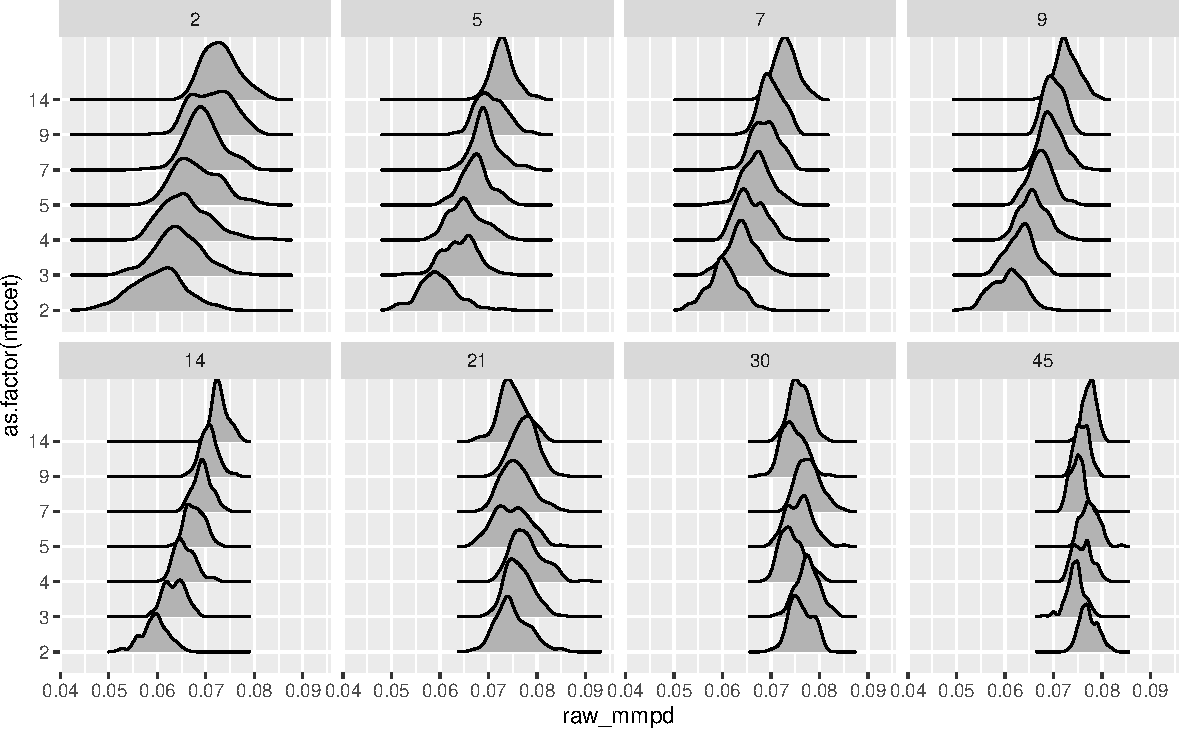
\includegraphics[width=\textwidth]{figure/dist-across-facets-1} 

}

\caption{Distribution of $MMPD_{raw}$ for different facet levels are shown. The location of the distribution shifts rightwards implying that as the number of facets increase, it is more likely that a higher value of $MMPD_{raw}$ will be obtained. }\label{fig:dist-across-facets}
\end{figure}

\begin{figure}

{\centering 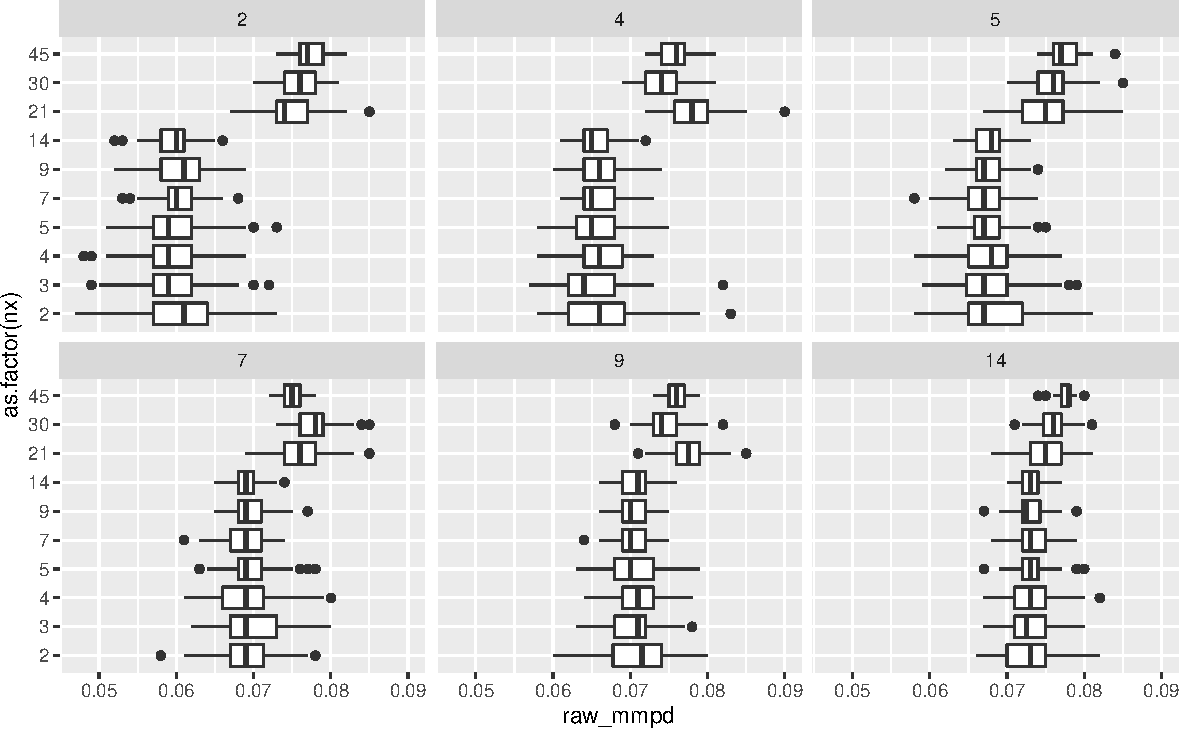
\includegraphics[width=\textwidth]{figure/dist-across-x-1} 

}

\caption{Distribution of $MMPD_{raw}$ for different x levels are shown. The scale of the distribution becomes less and less implying that as the number of x levels increase, it is more likely that a higher value of $MMPD_{raw}$ will be obtained as the spread of the distribution decreases. }\label{fig:dist-across-x}
\end{figure}

\hypertarget{normalisation}{%
\section{Normalisation}\label{normalisation}}

In an attempt to make the densities \ref{fig:hist_plot} same across different levels, we want to start by making their scale and location same. In that regard, we shuffle the data multiple times and compute the sampling distribution of \(mmpd_{raw}\) for each combination of facet and x-axis levels.

The null hypothesis is that the two cyclic granularities do not differ on the outcome (i.e., that the outcome is observed independently of treatment assignment). When we permute the outcome values during the test, we therefore see all of the possible alternative treatment assignments we could have had and where the mean-difference in our observed data falls relative to all of the differences we could have seen if the outcome was independent of treatment assignment. While a permutation test requires that we see all possible permutations of the data (which can become quite large), we can easily conduct ``approximate permutation tests'' by simply conducting a vary large number of resamples. That process should, in expectation, approximate the permutation distribution.

Finally, we run some simulation experiments to see if normalisation works. If normalisation has worked, it should work for both x levle and facet-levels.

Thus these median maximum pairwise distances need to be normalized for different harmonies in a way that eliminates the effect of different levels, consequently enabling comparison across different harmonies. The Fisher--Tippett--Gnedenko theorem in the field of Extreme Value Theory states that the maximum of a sample of iid random variables after proper re-normalization can converge in distribution to only one of Weibull, Gumbel or Freschet distribution, independent of the underlying data or process.

\hypertarget{methodology}{%
\subsection{Methodology}\label{methodology}}

The mean and sd for each combination of facet and x levels could be computed by shuffling the data repeatedly and obtaining the distribution of \(MMPD_{raw}\) for different combinations. If \(MMPD_{raw}\) is then adjusted by the location and scale of this distribution, we could assume that the distribution of the resultant \(MMPD_{norm}\) will have same distribution across different combinations of x and facet levels. All data is repeatedly shuffled \(nperm\) times in random manner to obtain the measure \(MMPD_{raw}\). Then the \(MMPD_{norm}\) is obtained by scaling the observed value by the mean and sd of the distribution of \(MMPD_{raw}\) obtained from the permuted data.

\noindent Step 7 in the Algorithm defined in Section \ref{sec:} need to be revised in order to compute \(MMPD_{norm}\) instead of \(MMPD_{raw}\). Step 1-6 stays the same. The entire algorithm will have to repeated for all harmony pairs considered in the context.

A simulation study is conducted to see if this methodology is working.

\hypertarget{simulation-study}{%
\subsection{Simulation study}\label{simulation-study}}

The behavior of the measure is monitored and understood through simulation experiments. A single simulation consisting of computational operations on a panel generating MMPD the value of which represents to what extent a pair of cyclic granularities would be interesting when displayed in the design. In comparing different simulation runs, we distinguish between different distributions and simulation scenarios (also iterations may be).

\hypertarget{simulated-designs}{%
\subsubsection{Simulated designs}\label{simulated-designs}}

D1. Same distribution of the measured variable across all x-axis and facet categories
D2. Different distribution across facet categories but same across x-axis categories
D3. Different distribution across x-axis categories but same across facet categories
D4. Different across both x-axis and facet categories

Each of these case scenarios tried against Normal and a non-normal (Gamma) distribution to check if underlying distribution has a role to play.

\hypertarget{environment}{%
\subsubsection{Environment}\label{environment}}

R version 4.0.1 (2020-06-06) is used with platform: x86\_64-apple-darwin17.0 (64-bit) running under: macOS Mojave 10.14.6

\hypertarget{experimental-set-up}{%
\subsubsection{Experimental set up}\label{experimental-set-up}}

This section describes the design of simulation runs, in terms of the scenarios simulated, the number of permutations used to compute estimates and to display the distribution of MMPD.

\begin{center}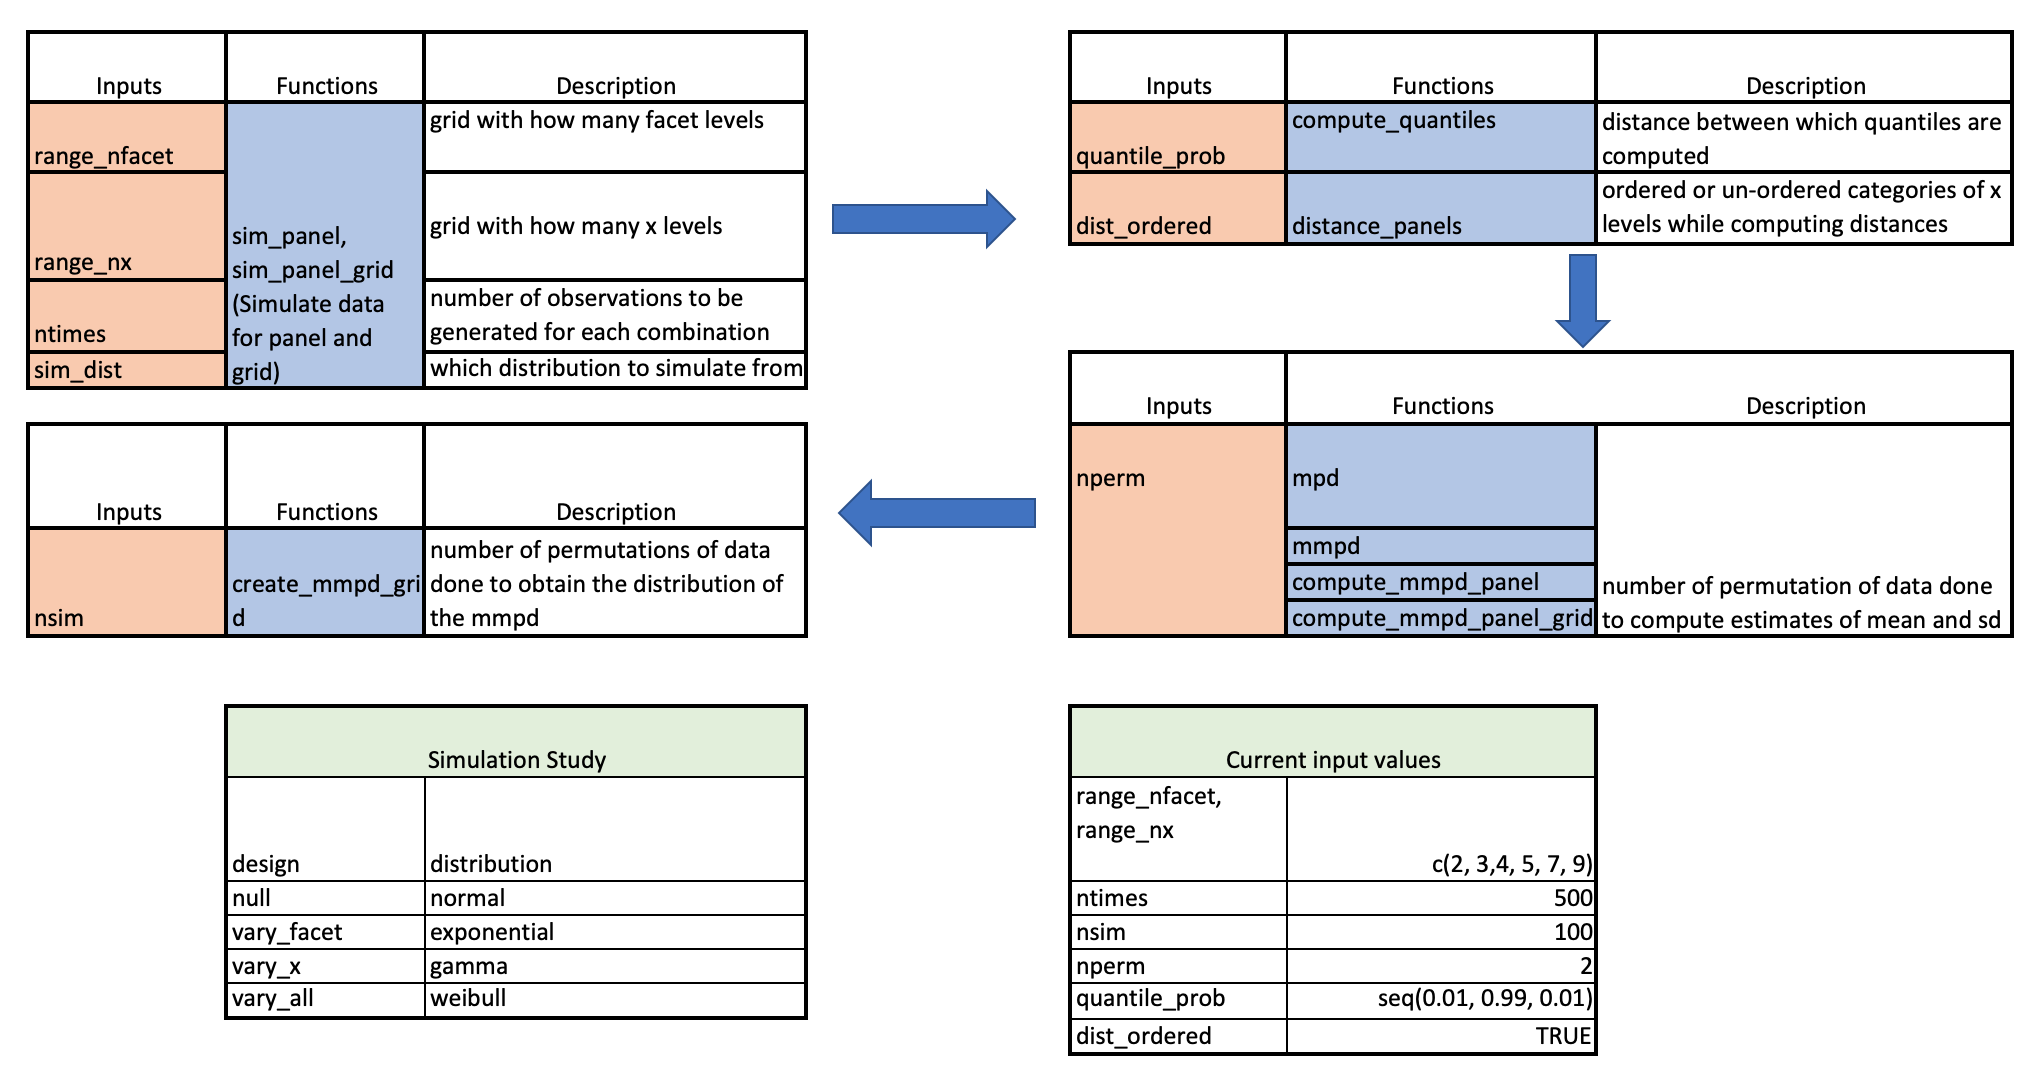
\includegraphics[width=\textwidth]{Figs/simulation} \end{center}

Observations from the null distribution are chosen as:\\
\texttt{sim\_norm\_null\ =\ \ \ distributional::dist\_normal(5,\ 10)}~\\
\texttt{sim\_gamma\_null\ \ =\ \ \ distributional::dist\_gamma(0.5,\ 0.2)}~\\

\hypertarget{results}{%
\subsection{Results}\label{results}}

\hypertarget{null-distribution}{%
\subsubsection{Null distribution}\label{null-distribution}}

Under the null hypothesis, all the combinations of x-axis and facets are obtained from the same distribution. We need to study the distribution of the mmpd values under the null hypothesis to see if comparison of their values across different x-axis and facet levels are at all possible. So, in turn it needs to be checked that if normalisation worked.

Currently, we see in Figure \ref{fig:null-dist} that the normalisation works fine for each facet since the distributions for each column are equal irrespective of the distribution type. But it does not work along the x-axis.

\begin{center}\includegraphics[width=\textwidth]{figure/norm-data, "Distribution of $MMPD_{norm}$ across different levels of facet and x-axis. These distributions should look the same if normalisation worked."-1} \end{center}

\begin{figure}

{\centering 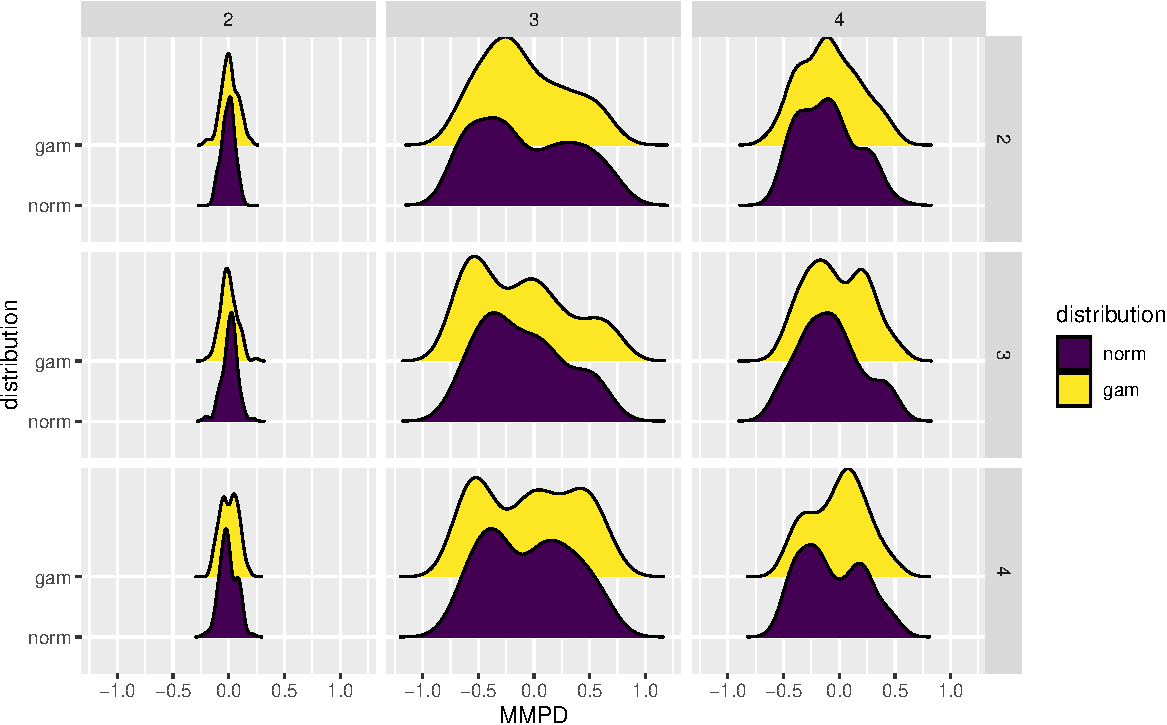
\includegraphics[width=\textwidth]{figure/null-dist-1} 

}

\caption{Distribution of mmpd across different facet levels (columns) and x-axis levels (rows) for null ditribution normal(5,10) and gamma(0.5, 0.2). The distribution of MMPD is unaffected by the null distribution considered. It is also the same across all facet levels but not across the x-axis, which means normalisation is failing across x-axis.}\label{fig:null-dist}
\end{figure}

\hypertarget{performance-of-normalised-mmpd}{%
\subsubsection{Performance of normalised MMPD}\label{performance-of-normalised-mmpd}}

\hypertarget{the-statistical-test}{%
\section{The statistical test}\label{the-statistical-test}}

\hypertarget{algorithm-1}{%
\subsection{Algorithm}\label{algorithm-1}}

for computation for all harmony pairs

\textbf{Assumption:} random permutation without considering ordering
(global)

\begin{enumerate}
\def\labelenumi{\arabic{enumi}.}
\item
  Given the data; \(\{v_t: t=0, 1, 2, \dots, T-1\}\), the MMPD is computed and is represented by \(MMPD_{obs}\).
\item
  From the original sequence a random permutation is obtained: \(\{v_t^*: t=0, 1, 2, \dots, T-1\}\).
\item
  MMPD is computed for all random permutation of the data and is represented by \(MMPD_{sample}\).
\item
  Steps (2) and (3) are repeated a large number
  of times M (e.g.~1000).
\item
  For each permutation, one \(MMPD_{sample}\) value is obtained.
\item
  \(95^{th}\) percentile of this \(MMPD_{sample}\) distribution is computed and stored in \(MMPD_{threshold}\).
\item
  If \(MMPD_{obs}> MMPD_{threshold}\), harmony pairs are accepted. Only one threshold for all harmony pairs.
\end{enumerate}

Pros: Considering thresholds global for all harmony pairs would imply less computation time.

Cons: Only one threshold for all harmony pairs means we are assuming distribution of all harmonies pairs are similar, which might not be the case.But nevertheless, it is a good benchmark.

\hypertarget{size-power-and-confidence-interval}{%
\subsection{Size, power and confidence interval}\label{size-power-and-confidence-interval}}

\hypertarget{characteristics-under-different-simulation-designs}{%
\paragraph{Characteristics under different simulation designs}\label{characteristics-under-different-simulation-designs}}

A set of simulation runs that are conducted and some outputs of which are reported.

\begin{center}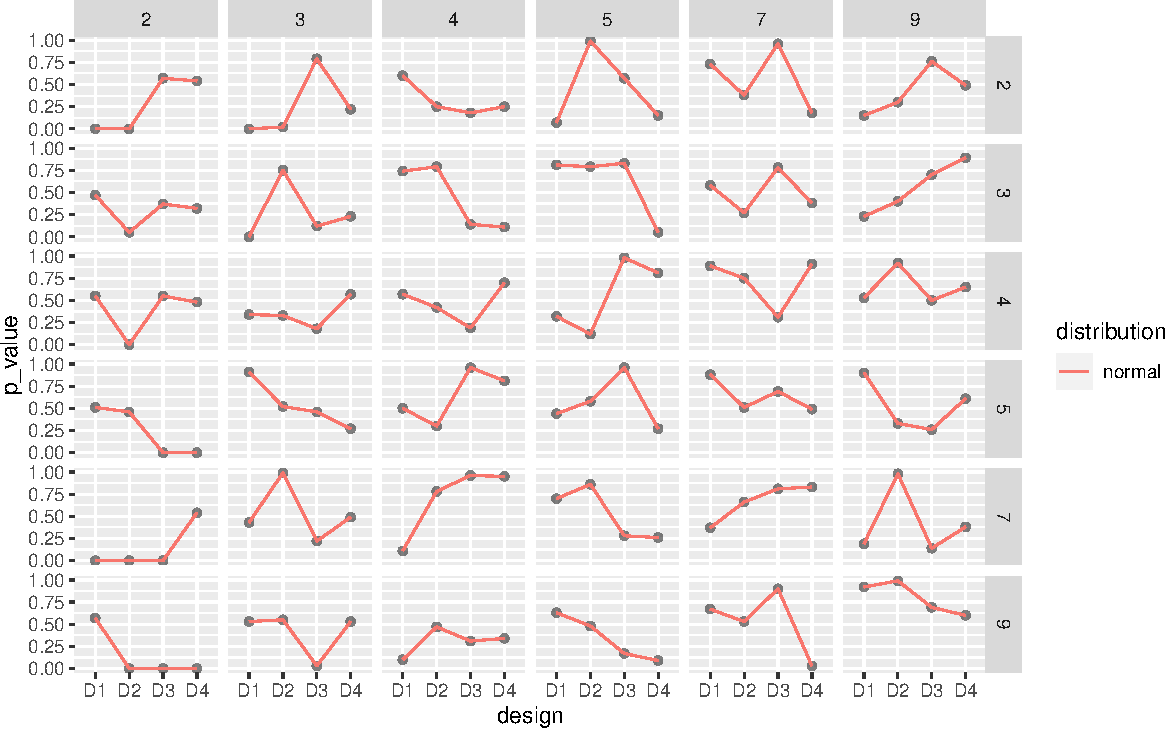
\includegraphics[width=\textwidth]{figure/sim_all-1} 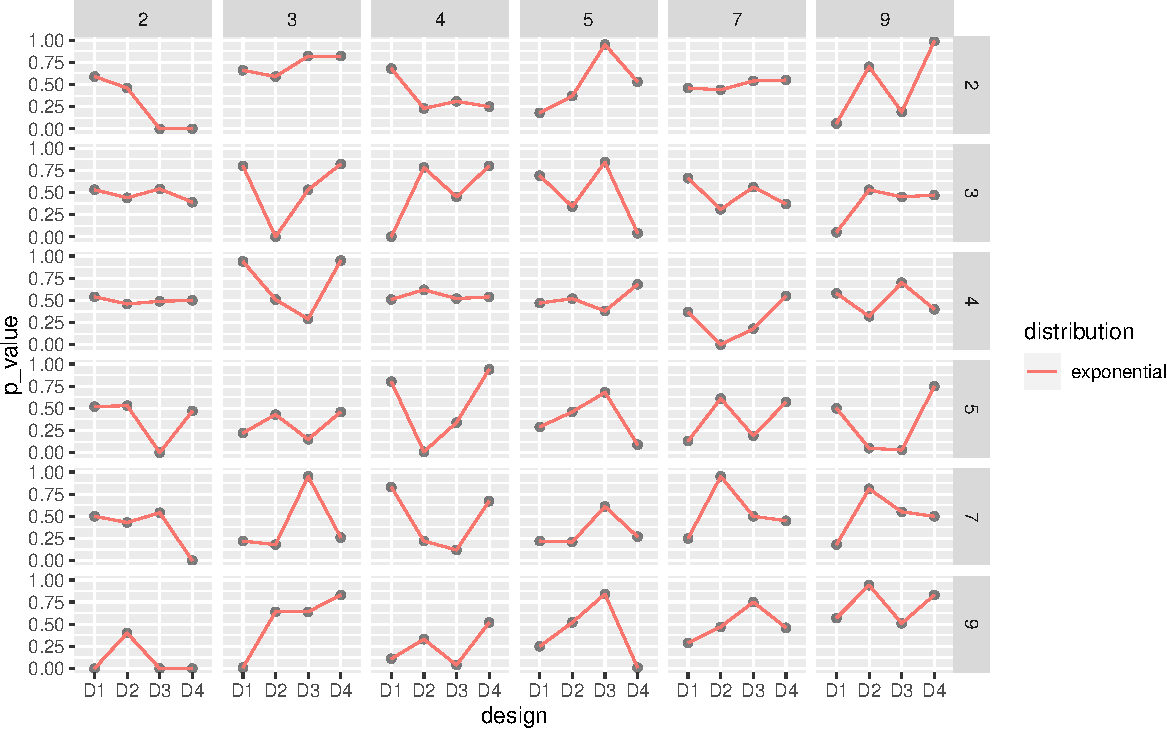
\includegraphics[width=\textwidth]{figure/sim_all-2} 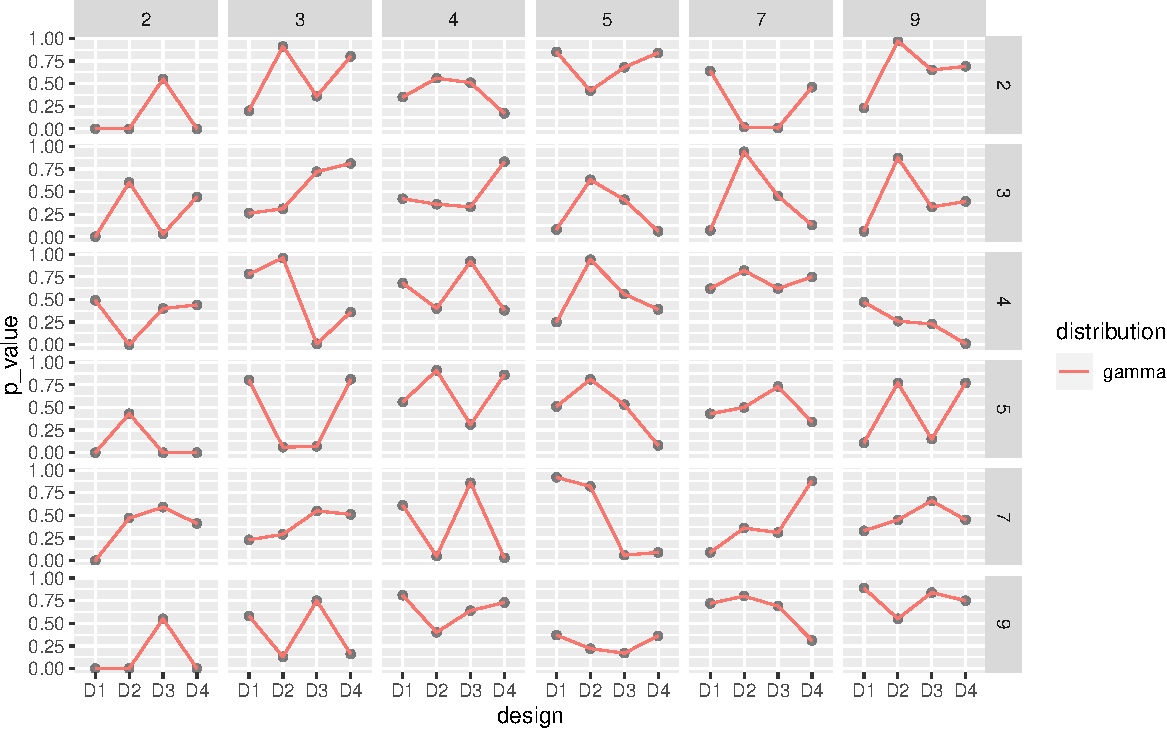
\includegraphics[width=\textwidth]{figure/sim_all-3} 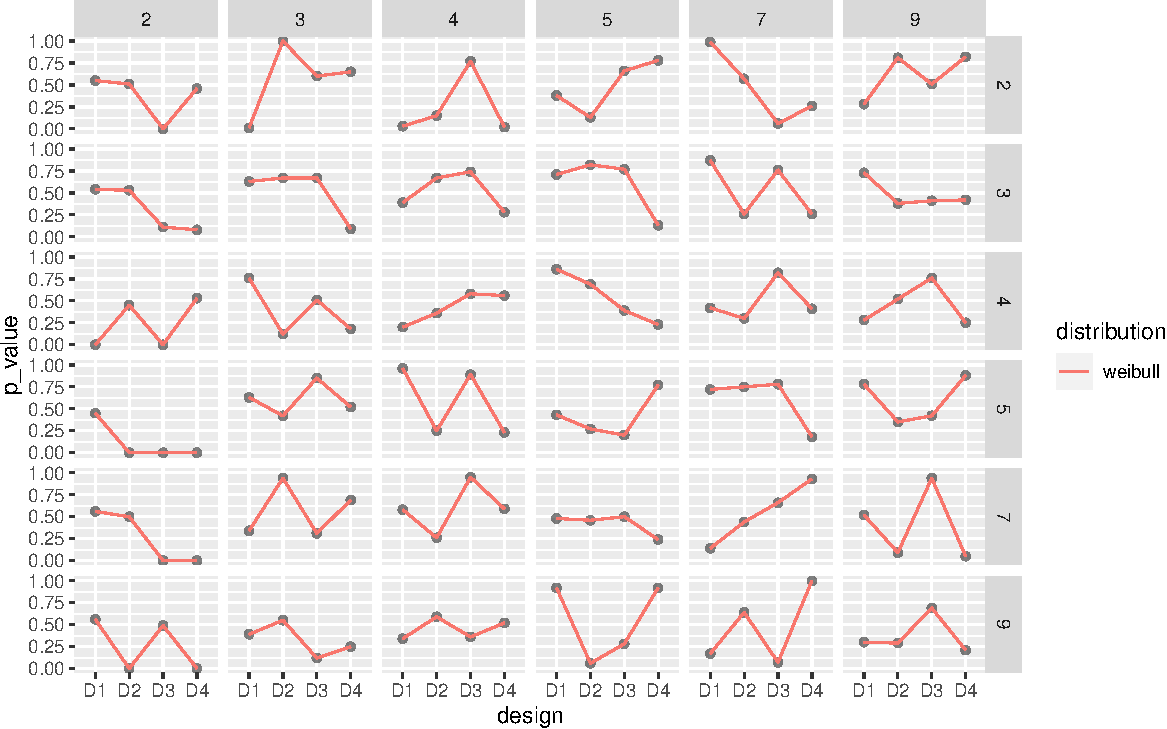
\includegraphics[width=\textwidth]{figure/sim_all-4} \end{center}

\hypertarget{algorithm-2}{%
\section{Algorithm}\label{algorithm-2}}

\noindent The algorithm employed for computing MMPD is summarized as follows:

\begin{itemize}
\tightlist
\item
  \textbf{Input:} Data corresponding to all harmony pairs, i.e., data sets of the form \((C_i, C_j, v)\)
  \(\forall i, j \in N_C\)\\
\item
  \textbf{Output:} MMPD (Median Maximum Pairwise Distances) measuring the average variation across different levels of \(C_i\) and \(C_j\) \(\forall i, j \in N_C\)
\end{itemize}

\begin{enumerate}
\def\labelenumi{\arabic{enumi}.}
\item
  Fix harmony pair \((C_i, C_j)\).
\item
  Fix \(k\). Then there are \(L\) groups corresponding to level \(A_k\) of \(C_i\).
\item
  Compute \(m = \binom{L}{2}\) pairwise distances between distributions of \(L\) unordered levels and \(m = L-1\) pairwise distances for \(L\) ordered categories.
\item
  Identify maximum within the \(m\) computed distances.
\item
  Compute normalized maximum distance (\(NM\)) using appropriate norming constants.
\item
  Use Steps 1-5 to compute normalized maximum distance for \(\forall k \in \{1, 2, \ldots, K\}\).
\item
  Compute MMPD = median \((NM_1, NM_2, \dots, NM_K)\)/log(\(K\)).
\item
  Repeat Steps 1 to 7 for all harmony pairs.
\end{enumerate}

\hypertarget{sec:application}{%
\section{Applications}\label{sec:application}}

\hypertarget{sec:smartmeter}{%
\subsection{Smart meter data of Australia}\label{sec:smartmeter}}

Smart meters provide large quantities of measurements on energy usage for households across Australia. One of the customer trials (Department of the Environment and Energy 2018) conducted as part of the Smart Grid Smart City project in Newcastle, New South Wales and some parts of Sydney provides customer wise data on energy consumption for every half hour from February 2012 to March 2014. The idea here is to show how to visualize the distribution of the energy consumption across different cyclic granularities in a systematic way to identify different behavioral patterns.

\hypertarget{cyclic-granularities-search-and-computation}{%
\subsubsection{Cyclic granularities search and computation:}\label{cyclic-granularities-search-and-computation}}

The tsibble object \texttt{smart\_meter10} from R package \texttt{gravitas} (Gupta et al. 2019) consisting of \texttt{reading\_datetime}, \texttt{customer\_id} and \texttt{general\_supply\_kwh} denoting the index, key and measured variable of the tsibble is used to facilitate the systematic exploration. While trying to explore the energy behavior of these customers systematically across cyclic time granularities, the first thing to consider is which cyclic time granularities we can look at exhaustively. Let us consider conventional time deconstructions for a Gregorian calendar (second, minute, half-hour, hour, day, week, month, year). Since the interval of this tsibble is 30 minutes, the temporal granularities may range from half-hour to year. Considering \(6\) linear granularities half-hour, hour, day, week, month and year in the hierarchy table, \(N_C = (6*5/2) = 15\). If \(N_C\) seem too large, the smallest and largest linear granularities could be considered to be removed from the hierarchy table. We remove half-year and year to have \(N_C = (4*3/2) = 6\) and obtain cyclic granularities namely ``hour\_day'', ``hour\_week'', ``hour\_month'', ``day\_week'', ``day\_month'' and ``week\_month'', read as ``hour of the day'', etc. Further, we add cyclic granularity day-type( ``wknd\_wday'') to capture weekend and weekday behavior. Now that we have a list of cyclic granularities to look at, we should be able to compute the multiple-order-up granularities using Section \ref{sec:cyclic-calendar}.

\hypertarget{screening-and-visualizing-harmonies}{%
\subsubsection{Screening and visualizing harmonies}\label{screening-and-visualizing-harmonies}}

From the search list, \(N_C = 7\) cyclic granularities are chosen for which we would like to derive insights of energy behavior. Recalling the data structure \textless{}\(C_i\), \(C_j\), \texttt{general\_supply\_kwh}\textgreater{} for exploration \(\forall i, j \in \{1, 2, \ldots, 7\}\), each of these \(7\) cyclic granularities can either be mapped to x-axis or to facet. Choosing \(2\) of the possible \(7\) granularities, which is equivalent to having \(^{7}P_2 = 42\) candidates for visualization. Fortunately, harmonies can be identified among those \(42\) possibilities to narrow the search. \autoref{tab:harmony-tab} shows \(16\) harmony pairs after removing clashes and any cyclic granularities with levels more than \(31\), as effective exploration becomes difficult with many levels (Section \ref{sec:levels}). The MMPD is also shown along with indicator (*) only when variation of measured variable across the harmony pair significant. Starting from \(42\) possible pairs of cyclic granularities to visualize, we are finally left with only \(6\), which is a very sizable number of displays for exploration.

Few harmony pairs are displayed in \autoref{fig:bothcust} to illustrate the significance of MMPD, threshold and the impact of different distribution plots and reverse mapping.
\noindent For each of \autoref{fig:bothcust} (b) and (c), \(C_i\) is the circular granularity day-type (weekday/weekend) and \(C_j\) is hour of the day. The geometry used for displaying the distribution is chosen as area-quantiles and violins in \autoref{fig:bothcust} (b and c respectively). \autoref{fig:bothcust} (a) displays reverse mapping of \(C_i\) and \(C_j\) with \(C_i\) denoting hour of the day and \(C_j\) denoting day-type with distribution geometrically displayed as boxplots.

In \autoref{fig:bothcust} (b), the black line is the median, whereas the purple band covers 25th to 75th percentile, the orange band covers 10th to 90th percentile and the green band covers 1st to 99th percentile. The first facet represents the weekday behavior while the second one displays the weekend behavior and energy consumption across each hours of the day is shown inside each facet. The energy consumption is extremely (positive- or right-) skewed with the 1st, 10th and 25th percentile lying relatively close whereas 75th, 90th and 99th lying further away from each other. This is common across both weekdays and weekends. For the first few hours on weekdays, median energy consumption starts and continues to be higher for longer as compared to weekends.

Consider looking at violin plots instead of quantile plots to look at the same data in \autoref{fig:bothcust}(c). There is additional information that we can derive looking at the distribution. There is bimodality in the early hours of the day, implying both low and high energy consumption is probable in the early hours of the day both for weekdays and weekends. If we visualize the same data with reverse mapping of the cyclic granularities, then the natural tendency would be to compare weekend and weekday behavior within each hour and not across hours. For example in \autoref{fig:bothcust}(a), it can be seen that median energy consumption for the early morning hours is extremely high for weekdays compared to weekends. Also, outliers are more prominent in the latter part of the day. All of these indicate that looking at different distribution geometry or changing the mapping might shed lights on different aspect of the energy behavior for the same sample population.

\begin{figure}

{\centering 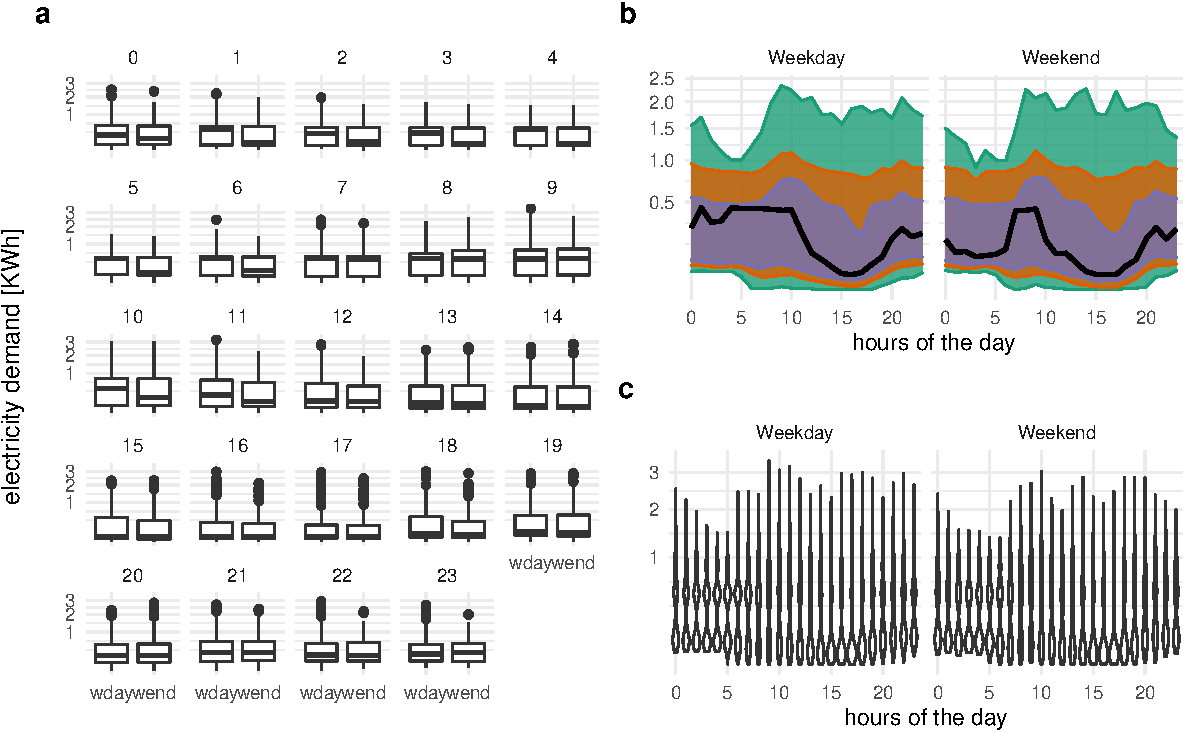
\includegraphics[width=0.9\linewidth]{figure/bothcust-1} 

}

\caption{Energy consumption of a single customer shown with different distribution displays, and granularity arrangements. Two granularities are used: hour of the day (I) and weekday/weekend (II). Plot (a) shows granularity I facetted by granularity II, and plots (b), (c) shows the converse mapping. Plot (a) makes a comparison of usage by workday within each hour of the day using side-by-side boxplots. Generally, on a work day there is more consumption early in the day.  Plots (b) and (c) examine the temporal trend of consumption over the course of a day, separately for the type of day. Plot (b) uses an area quantile to put the emphasis on the time series, for example, the median consumption over time shows prolonged usage in the morning on weekdays. Plot (c) uses a violin plot to place emphasis on distributional differences across hours. It can be seen that the morning use on weekdays is bimodal, some work days there is low usage, which might indicate the person is working from home and also having a late start.}\label{fig:bothcust}
\end{figure}

If the data for all keys are visualized together, it might lead to Simpson's paradox, which occurs when one observation shows a particular behavior, but this behavior paradoxically becomes obscured by aggregation. For example in a particular neighborhood one household may have the least daily power consumption for a full week, yet still not be the household with the minimum weekly power consumption. This is an intuitive possibility, because heterogeneous \texttt{customer\_id}'s with very different occupation or demographics will tend to have very different energy behavior and combining them together will somehow weaken any typical or extreme behavior. A strategy for analyzing multiple keys together could be to first group them basis time series or demographic features and then look at their energy behavior. This is beyond the scope of the current work.

This case study shows systematic exploration of energy behavior for a household to gain exhaustive insights on periodic behavior of the households.

\hypertarget{sec:cricket}{%
\subsection{T20 cricket data of Indian Premiere League}\label{sec:cricket}}

The method is not only restricted to temporal data, and can be generalized to many hierarchical granularities (with continuous and uni-directional nature). We illustrate this with an application to the sport cricket. Although there is no conventional time component in cricket, each ball can be thought to represent an ordering from past to future with the game progressing forward with each ball. In the Twenty20 format, an over will consist of 6 balls (with some exceptions), an inning is restricted to a maximum of 20 overs, a match will consist of 2 innings and a season consists of several matches. Thus, similar to time, there is a hierarchy where ball is nested within overs, overs nested within innings and innings within matches. The idea of cyclic granularities can be likewise mapped to this hierarchy. Example granularites then include ball of the over, over of the inning and ball of the inning. Although most of these cyclic granularities are circular in design of the hierarchy, in application of the rules some granularities are aperiodic. For example, in most cases an over will consist of 6 balls with some exceptions like wide balls or when an inning finishes before the over finishes. Thus, the cyclic granularity ball-of-over will be circular in most cases and aperiodic in others.

The Indian Premier League (IPL) is a professional Twenty20 cricket league in India contested by eight teams representing eight different cities in India. The ball by ball data for IPL season 2008 to 2016 is fetched from \href{https://www.kaggle.com/josephgpinto/ipl-data-analysis/data}{Kaggle}. The \texttt{cricket} data set in the \texttt{gravitas} package summarizes the ball-by-ball data across overs and contains information for a sample of 214 matches spanning 9 seasons (2008 to 2016) such that each over has 6 balls, each inning has 20 overs and each match has 2 innings. This could be useful in a periodic world when we wish to compute any circular/quasi-circular granularity based on a hierarchy table which look like \autoref{tab:hierarchy-cric}.

\begin{table}

\caption{\label{tab:hierarchy-cric}Hierarchy table for cricket where overs are nested within an inning, innings nested within a match and matches within a season.}
\centering
\begin{tabular}[t]{lll}
\toprule
linear (G) & single-order-up cyclic (C) & period length/conversion operator (K)\\
\midrule
over & over-of-inning & 20\\
inning & inning-of-match & 2\\
match & match-of-season & k(match, season)\\
season & 1 & 1\\
\bottomrule
\end{tabular}
\end{table}

However, even if the situation is not periodic and a similar hierarchy can not be formed, it can be interesting to visualize the distribution of a measured variable across relevant cyclic granularities to shed light on the aperiodic behavior of a non-temporal data set similar to aperiodic events like formal meetings, workshops, conferences, school semesters in a temporal set up. There are many interesting questions that could possibly be answered with such a data set irrespective of the type of cyclic granularities.

First, it would be interesting to see if the distribution of total runs vary depending on if a team bats in the first or second innings. The Mumbai Indians (MI) and Chennai Super kings (CSK) appeared in final playoffs from 2010 to 2015. We take their example in order to dive deeper into this question. From Figure \ref{fig:cricex}(a), it can be observed that for the team batting in the first inning there is an upward trend of runs per over, while there is no clear upward trend in median and quartile deviation of runs for the teams batting in the second inning. This seem to indicate that players feel mounting pressure to score more runs as they approach towards the end of the first inning. Whereas teams batting in the second inning have a set target in mind and are not subjected to such mounting pressure and may adopt a more conservative strategy, to score runs. Thus winning teams like CSK and MI seem to employ different inning strategies when it comes to their batting order.

Another interesting question could be: do runs per over decrease in the subsequent over if fielding (defending) was good in the previous over? For establishing the fielding quality, we apply an indicator function on dismissals (1 if there was at least one wicket in the previous over due to run out or catch, 0 otherwise). Runs in the current over is then the observation variable. Dismissals in the previous over can lead to a batsman adopting a more defensive play style. Figure \ref{fig:cricex}(b) shows that no dismissals in the previous over leads to a higher median and quartile spread of runs per over as compared to the case when there has been at least one dismissal in the previous over.

\begin{figure}

{\centering 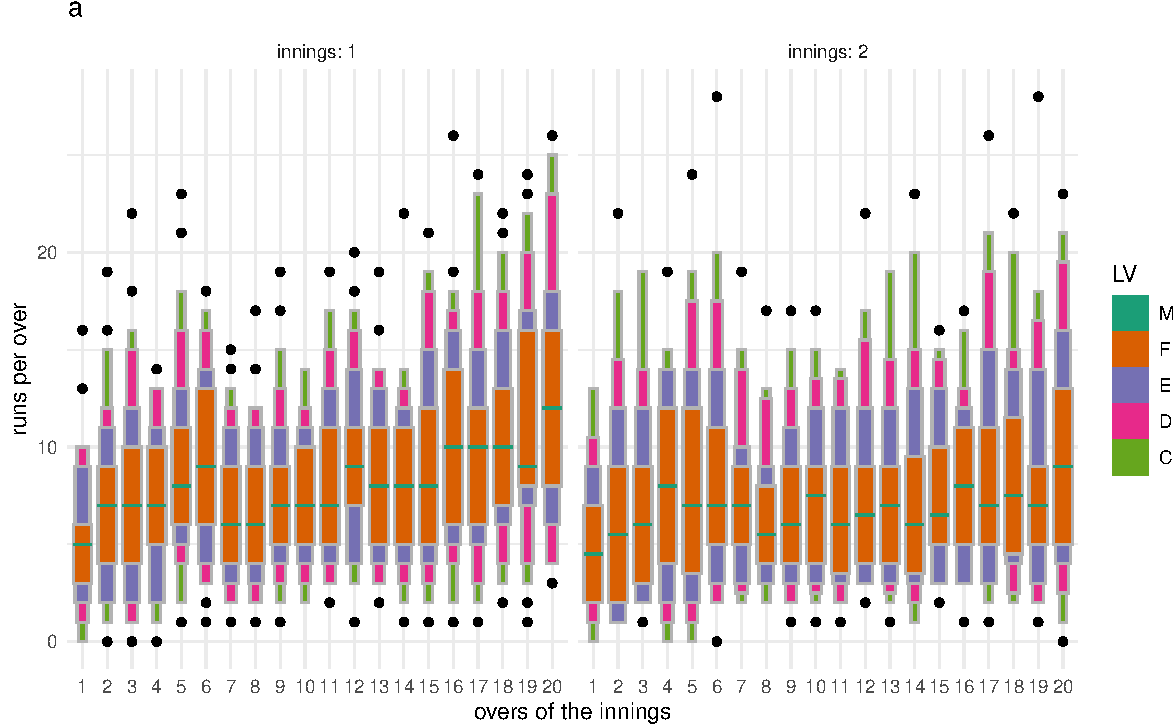
\includegraphics[width=0.9\linewidth]{figure/cricex-1} 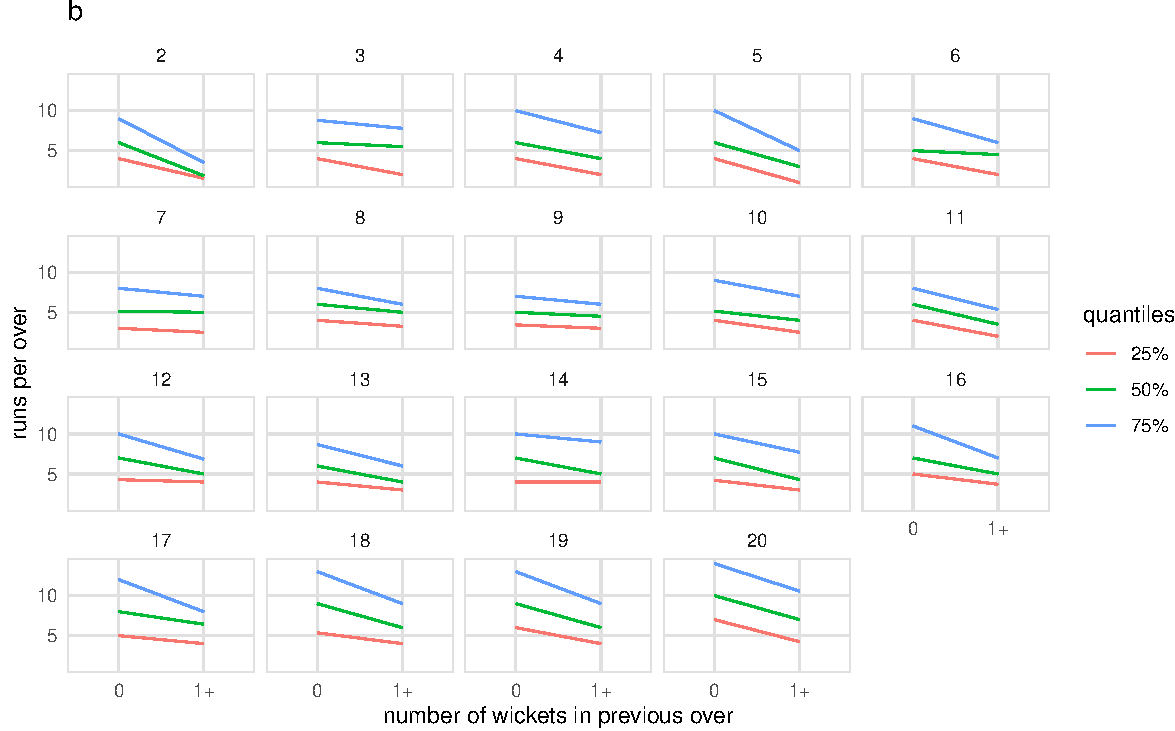
\includegraphics[width=0.9\linewidth]{figure/cricex-2} 

}

\caption{Runs per over shown with different distribution displays, and granularities. Plot (a) shows letter value plot across overs faceted by innings. For the team batting in the first innings there is an upward trend of runs per over, while there is no such pattern of runs for the teams batting in the second innings. Plot (b) shows quantile plot of runs per over across an indicator of wickets in previous over faceted by current over. This indicates that at least one wicket in the previous over leads to lower median run rate and quartile spread in the subsequent over.}\label{fig:cricex}
\end{figure}

Wickets per over are considered as an aperiodic cyclic granularity with wickets as an aperiodic linear granularity. These granularities do not appear in the hierarchy table since it is difficult to position them in a hierarchy. These are similar to holidays or special events in temporal data.

\hypertarget{discussion-points-and-future-work}{%
\section{Discussion points and future work}\label{discussion-points-and-future-work}}

Exploratory data analysis involve many iterations of finding and summarizing patterns. With temporal data available at ever finer scales, exploring periodicity has become overwhelming with so many possible granularities to explore. This work refines the selection of appropriate pairs of granularities by identifying those for which the differences between the displayed distributions is greatest, and rating these selected harmony pairs in order of importance for exploration.

A future direction of work could be to look at more individuals/subjects and group them according to similar periodic behavior. Behaviors across different cyclic granularities would be different for different subjects and one way to find groups would be to actually locate clusters who have similar periodic behavior.

\hypertarget{appendix}{%
\section{Appendix}\label{appendix}}

\hypertarget{null-distribution-1}{%
\subsection{Null distribution}\label{null-distribution-1}}

\hypertarget{size-simulated-same-distribution-for-all-combinations-of-categories-for-all-harmony-pairs.}{%
\subsubsection{Size: Simulated same distribution for all combinations of categories for all harmony pairs.}\label{size-simulated-same-distribution-for-all-combinations-of-categories-for-all-harmony-pairs.}}

Failure to reject the null hypothesis when there is in fact no significant effect.

\hypertarget{normalised-maximum-distances-follow-standard-gumbel-distribution}{%
\subsubsection{Normalised maximum distances follow standard Gumbel distribution}\label{normalised-maximum-distances-follow-standard-gumbel-distribution}}

\hypertarget{limiting-distribution-of-median-of-normalised-maximum-distances-is-normal}{%
\subsubsection{Limiting distribution of median of normalised maximum distances is normal}\label{limiting-distribution-of-median-of-normalised-maximum-distances-is-normal}}

Let a continuous population be given with cdf F(x) (cumulative distribution function) and median \(\xi\) (assumed to exist uniquely). For a sample of size \(2n + 1\), let \(\tilde{x}\) denote the sample median. The distribution of \(\tilde{x}\),under certain conditions, to be asymptotically normal with mean \(\xi\) and variance \(\sigma_n^2 = \frac{1}{4} [f(\xi)]^2(2n + 1)\), where \(f(x) = F'(x)\) is the pdf (probability density function).

\hypertarget{power}{%
\subsection{Power}\label{power}}

\hypertarget{confidence-interval}{%
\subsection{Confidence interval}\label{confidence-interval}}

Failure to reject the null hypothesis when there is in fact a significant effect.

To estimate the sampling distribution of the test statistic we need many samples generated under the null hypothesis. If the null hypothesis is true, changing the exposure would have no effect on the outcome. By randomly shuffling the exposures we can make up as many data sets as we like. If the null hypothesis is true the shuffled data sets should look like the real data, otherwise they should look different from the
real data. The ranking of the real test statistic among the shuffled test statistics gives a p-value.

\hypertarget{varying-distribution-across-facet}{%
\subsubsection{Varying distribution across facet}\label{varying-distribution-across-facet}}

\hypertarget{varying-distribution-across-x-axis}{%
\subsubsection{Varying distribution across x-axis}\label{varying-distribution-across-x-axis}}

\hypertarget{varying-distribution-across-both-facets-and-x-axis}{%
\subsubsection{Varying distribution across both facets and x-axis}\label{varying-distribution-across-both-facets-and-x-axis}}

\hypertarget{repeat-all-with-varying-facet-and-x-axis-levels}{%
\subsubsection{Repeat all with varying facet and x-axis levels}\label{repeat-all-with-varying-facet-and-x-axis-levels}}

\emph{Conclusion}: The test should reject the null hypothesis if distributions are different.

\hypertarget{refs}{}
\leavevmode\hypertarget{ref-Dang2014-tw}{}%
Dang, T N, and L Wilkinson. 2014. ``ScagExplorer: Exploring Scatterplots by Their Scagnostics.'' In \emph{2014 IEEE Pacific Visualization Symposium}, 73--80.

\leavevmode\hypertarget{ref-smart-meter}{}%
Department of the Environment and Energy. 2018. \emph{Smart-Grid Smart-City Customer Trial Data}. Australian Government, Department of the Environment; Energy: Department of the Environment; Energy, Australia. \url{https://data.gov.au/dataset/4e21dea3-9b87-4610-94c7-15a8a77907ef}.

\leavevmode\hypertarget{ref-R-gravitas}{}%
Gupta, Sayani, Rob Hyndman, Di Cook, and Antony Unwin. 2019. \emph{gravitas: Explore Probability Distributions for Bivariate Temporal Granularities}. \url{https://CRAN.R-project.org/package=gravitas}.

\leavevmode\hypertarget{ref-Gupta2020-vo}{}%
Gupta, Sayani, Rob J Hyndman, Dianne Cook, and Antony Unwin. 2020. ``Visualizing Probability Distributions Across Bivariate Cyclic Temporal Granularities,'' October. \url{http://arxiv.org/abs/2010.00794}.

\leavevmode\hypertarget{ref-Kullback1951-jy}{}%
Kullback, S, and R A Leibler. 1951. ``On Information and Sufficiency.'' \emph{Ann. Math. Stat.} 22 (1): 79--86.

\leavevmode\hypertarget{ref-Menendez1997-in}{}%
Menéndez, M L, J A Pardo, L Pardo, and M C Pardo. 1997. ``The Jensen-Shannon Divergence.'' \emph{J. Franklin Inst.} 334 (2): 307--18.

\leavevmode\hypertarget{ref-tukey1988computer}{}%
Tukey, John W, and Paul A Tukey. 1988. ``Computer Graphics and Exploratory Data Analysis: An Introduction.'' \emph{The Collected Works of John W. Tukey: Graphics: 1965-1985} 5: 419.

\leavevmode\hypertarget{ref-wang2020calendar}{}%
Wang, Earo, Dianne Cook, and Rob J Hyndman. 2020. ``Calendar-Based Graphics for Visualizing People's Daily Schedules.'' \emph{Journal of Computational and Graphical Statistics}. \url{https://doi.org/10.1080/10618600.2020.1715226}.

\leavevmode\hypertarget{ref-wilkinson2005graph}{}%
Wilkinson, Leland, Anushka Anand, and Robert Grossman. 2005. ``Graph-Theoretic Scagnostics.'' In \emph{IEEE Symposium on Information Visualization, 2005. INFOVIS 2005.}, 157--64. IEEE.

\end{document}
